% \documentclass{article}

\documentclass{article}
%% \documentclass[twocolumn]{article}

\renewcommand{\familydefault}{\sfdefault} % Standardfont ändern auf Sans Serif (bny)

\usepackage[utf8x]{inputenc}
\usepackage[german]{babel} % Sprache umschalten /hat funktioniert bis auf Authors, bny 13.04.2016
\usepackage{tcolorbox}
\usepackage{xcolor}
\definecolor{chamois}{rgb}{1,.984314,.956863}  % RGB 255 247 231
\pagecolor{chamois}
\usepackage{geometry}
\usepackage{eurosym}
\geometry{verbose,a4paper,tmargin=10mm,bmargin=10mm,lmargin=10mm,rmargin=10mm}
\usepackage[T1]{fontenc}

\usepackage{multicol} % 20.04.2017 hinzugefügt, bny

%%% \usepackage{tikz}
%%% % \pagecolor{olive!50!yellow!50!white}

%% --> Hinweis, 11.08.2017, bny
%% --> Multicol ist nur zuständig für Spalten, die farbigen Kacheln werden mit tcolorbox gemacht
%% --> soll nur eine einspaltige Box eingefügt werden, wird multicol auskommandiert. (siehe Beschaffung)

\tcbuselibrary{skins}

\colorlet{xlightblue}{blue!5}

\newtcolorbox{beamerlikethm}[1]{
  title=#1,
  beamer,
  % colback=xlightblue,
  colframe=red!50,
  fonttitle=\bfseries,
  left=1mm,
  right=1mm,
  top=1mm,
  bottom=1mm,
  middle=1mm
}


\begin{document}
\pagestyle{empty}

%%% \begin{tikzpicture}[remember picture, overlay]
%%% \shade[left color=red!50,
%%% right color=green!50
%%% ] (current page.north west) rectangle (current page.south east);
%%% \end{tikzpicture}

%%%%%%%%%%%%%%%%%%%%%%%%%%%%%%%
\centering{{\huge CUBE PA - Einführung}}

\vspace{\baselineskip}

%%%% Box 1+2 in zwei Spalten

\begin{multicols}{2}

\begin{tcolorbox}[colback=blue!5,colframe=blue!40!black,title=Die Menüführung]
\begin{itemize}
  \item[$\Longrightarrow$] Links sehen Sie sämtliche Module, welche für Sie freigeschaltet sind.
  \item[$\Longrightarrow$] Mit Klick oben links auf den Namen können Sie sich abmelden, das Passwort zurücksetzen und das Handbuch herunterladen.
\end{itemize}
\begin{centering}
\center{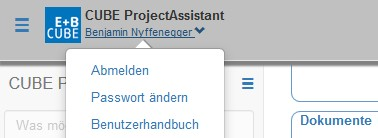
\includegraphics[width=.6\linewidth]{Pictures/Menu.jpg}}
\end{centering}
\begin{itemize}
  \item[$\Longrightarrow$] Mit Klick auf 
\includegraphics[height=12pt]{Icons/Menu_Aus-Ein.jpg} links des Emch+Berger Logos können Sie das Menü ein- und ausschalten. So gewinnen Sie eine grössere Arbeitsfläche.
	\item[$\Longrightarrow$] Arbeiten Sie mit mehreren Instanzen können Sie mit Klick auf 
\includegraphics[height=12pt]{Icons/Instanz_wechseln.jpg} rechts der Eingabezeile 'Was möchten Sie tun?' die Instanz wechseln.
\end{itemize}
\end{tcolorbox}




\begin{tcolorbox}[colback=blue!5,colframe=blue!40!black,title=Was möchten Sie tun?]
\begin{itemize}
  \item[$\Longrightarrow$] Geben Sie in die Zeile 'Was möchten Sie tun?' einen Suchbegriff ein. CUBE PA durchsucht nebst den Datenbankeinträgen, auch Dokumente und listet die Suchergebnisse auf.
  \item[$\Longrightarrow$] Wollen Sie ein neues Dokument erstellen, tippen Sie ins Feld 'Dok'. Die Option erscheint, ein neues Dokument zu erstellen.  Dasselbe funktioniert auch mit Pendenzen, Entscheiden und Beschaffungen.
	\item[$\Longrightarrow$] Alternativ können Sie ins Suchfeld 'Neu' schreiben. Wählen Sie den gewünschten Eintrag aus, welcher Sie neu anlegen wollen.
	\item[$\Longrightarrow$] Fahren Sie über ein Suchresultat, erscheinen die Optionen. Bei einem gefundenen Dokument können Sie sich dieses beispielsweise 'anzeigen' lassen, das Dokument 'herunterladen', oder 'bearbeiten'. 
\end{itemize}
\end{tcolorbox}


\end{multicols}

\begin{beamerlikethm}{Die persönliche Projektübersicht}
\begin{itemize}
 \item[$\Longrightarrow$] In der persönlichen Projektübersicht sehen Sie die für Sie relevanten Informationen.
 \item[$\Longrightarrow$] \textbf{Sitzungen:} Ihnen werden die nächsten Sitzungen mit der entsprechenden Sitzungseinladung angezeigt. Ebenso werden die vergangenen Sitzungen mit Link zum zugehörigen Protokoll aufgelistet.
 \item[$\Longrightarrow$] Rechts finden Sie die \textbf{Pendenzen}, für welche Sie verantwortlich sind. Mit Klick auf 
\includegraphics[height=10pt]{Icons/Pfeil_rechts.jpg} öffnen Sie die entsprechenden Pendenzen. Mit 
\includegraphics[height=10pt]{Icons/bearbeiten.jpg} können Sie eine Pendenz gleich bearbeiten.
 \item[$\Longrightarrow$] Bei der \textbf{Dokumentenübersicht} finden Sie die von Ihnen ausgecheckten Dokumenten. Zudem werden alle Dokumente angezeigt, welche sie favorisiert haben. Oft verwendete und gespeicherte Filter werden ebenfalls angezeigt und mit einem Klick wechseln Sie in die Dokumentenablage und erhalten das Filterergebnis.
 \item[$\Longrightarrow$] Bei der Übersicht über \textbf{Beschaffungen} werden die Beschaffungen angezeigt, bei welchen Sie Aufgaben wahrnehmen. So zum Beispiel bei der Vertragsüberwachung: Alle Verträge die von Ihnen begleitet werden, sehen Sie aufgelistet.
\end{itemize}
\end{beamerlikethm}

%%%% Box 3+4 in zwei Spalten

\begin{multicols}{2}

\begin{tcolorbox}[colback=blue!5,colframe=blue!40!black,title=Mobile CUBE PA Version]
\begin{itemize}
  \item[$\Longrightarrow$] CUBE PA lässt sich auch mittels App für iPhone und Android Smartphones bedienen.
  \item[$\Longrightarrow$] Sie können das Programm mittels AppShop gratis herunterladen.
  \item[$\Longrightarrow$] Melden Sie sich mit ihren bekannten Anmeldedaten an.
  \item[$\Longrightarrow$] Die App unterstützt die 'persönliche Übersicht', die 'Adressliste', das 'Sitzungswesen' sowie 'die Dokumentenablage.
	\item[$\Longrightarrow$] So haben Sie die wichtigesten Tools von CUBE PA jederzeit zur Hand und können auf Sitzungen und Dokumente, aber auch Adressen zugreifen.
\end{itemize}
\begin{centering}
\center{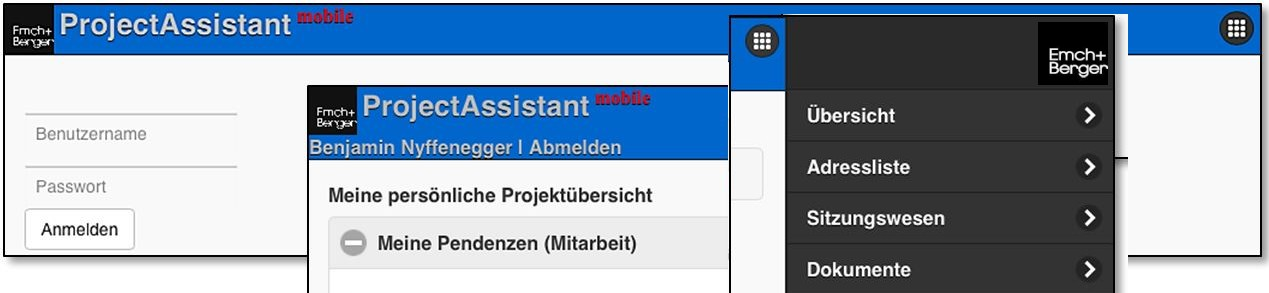
\includegraphics[width=1\linewidth]{Pictures/Mobile.jpg}}
\end{centering}
\end{tcolorbox}


\begin{tcolorbox}[colback=blue!5,colframe=blue!40!black,title=Die verfügbaren Module von CUBE PA]
\begin{itemize}
  \item[$\Longrightarrow$] Adresslisten und Terminplanung (Terminplan per pdf herunterladen oder MS Project-Terminplan importieren und filtern).
  \item[$\Longrightarrow$] Sitzungswesen mit Pendenz- und Entscheideverwaltung. Protokollieren Sie direkt in CUBE PA.
	\item[$\Longrightarrow$] Anforderungs- und Mängelmanagement zur Abnahme oder Begleitung von Projekten.
	\item[$\Longrightarrow$] Beschaffungswesen und Controlling für die Unterstützung bei Beschaffungen und Projekten.
		\item[$\Longrightarrow$] Qualitätsmanagement: Download von Sicherheitsdokumenten und Erstellung von Projektjournalen.
		\item[$\Longrightarrow$] CRM: Eventmanagement mit Einladungsorganisation und Webseite.
		\item[$\Longrightarrow$] Dokumentenablage: Dokumente überall und aktuell zur Hand, Versionifizierung, versenden und drucken via Reprozentrum.
\end{itemize}
\end{tcolorbox}


\end{multicols}


%%%%%%%%%%%%%%%%%%%%%


\pagebreak
\centering{{\huge Dokumentenablage}}

\vspace{\baselineskip}

%%%% Box 1+2 in zwei Spalten

\begin{multicols}{2}

\begin{tcolorbox}[colback=blue!5,colframe=blue!40!black,title=Dokumente hochladen]
\begin{itemize}
  \item[$\Longrightarrow$] Klicken Sie auf das 
\includegraphics[height=10pt]{Icons/Plussymbol.jpg}, die Eingabemaske öffnet sich.
  \item[$\Longrightarrow$] Ziehen Sie das gewünschte File in das Feld 'Datei' oder geben Sie einen Link in das Feld 'Adresse' ein.
  \item[$\Longrightarrow$] Füllen Sie die anderen Felder aus.
  \item[$\Longrightarrow$] Bevor Sie das Dokument mittels 
\includegraphics[height=12pt]{Icons/B_Erstellen.jpg} speichern können, müssen Sie noch mindestens eine Zugriffsberechtigung definieren. 
	\item[$\Longrightarrow$] Dazu klicken Sie auf 
\includegraphics[height=10pt]{Icons/Pluszeichen.jpg} und fügen (in der Regel) ihren Namen und die gewünschten Berechtigungen hinzu.
	\item[$\Longrightarrow$] Schliessen Sie den Vorgang nun mit 
\includegraphics[height=12pt]{Icons/B_Erstellen.jpg} ab.
\end{itemize}
\end{tcolorbox}


\begin{tcolorbox}[colback=blue!5,colframe=blue!40!black,title=Dokumente mit Google-Maps verknüpfen]
\begin{itemize}
  \item[$\Longrightarrow$] Wählen Sie das gewünschte Dokument aus und klicken Sie auf  
\includegraphics[height=10pt]{Icons/bearbeiten.jpg}.
  \item[$\Longrightarrow$] Klicken Sie oben rechts im Bearbeitungsfenster auf 'Karte anzeigen / verstecken'. Google-Maps wird nun angezeigt.
  \item[$\Longrightarrow$] Durch Klick auf die linke Maustaste können Sie den Kartenauschnitt verschieben; mittels einem Scroll-Rad können Sie die Karte vergrössern oder verkleinern.
  \item[$\Longrightarrow$] Haben Sie den gewünschten geographischen Ort gefunden, machen Sie dort mit der Maus einen Doppelklick. Es wird eine Nadel gesetzt: 
\includegraphics[height=10pt]{Icons/vNadel.jpg}.
	\item[$\Longrightarrow$] Sie können die 
\includegraphics[height=10pt]{Icons/vNadel.jpg} jederzeit wieder verschieben oder mittels Rechtsklick löschen.
\end{itemize}
\end{tcolorbox}


\end{multicols}

%%%% Box 3+4 in zwei Spalten

\begin{multicols}{2}

\begin{tcolorbox}[colback=blue!5,colframe=blue!40!black,title=Bearbeiten von Dokumenten]
\begin{itemize}
  \item[$\Longrightarrow$] Klicken Sie in der Dokumentenübersicht auf den Titel des gewünschten Dokuments. Es öffnen sich die Optionen.
  \item[$\Longrightarrow$] Klicken Sie auf 
\includegraphics[height=12pt]{Icons/Auschecken.jpg}. Das Dokument wird ausgeckeckt und im Word geöffnet.
  \item[$\Longrightarrow$] Bearbeiten Sie das Dokument und klicken Sie fürs Speichern 
\includegraphics[height=12pt]{Icons/Sync2013.jpg} oder 
\includegraphics[height=12pt]{Icons/Sync2016.jpg} oben links im Word. Das Dokument wird gleich wieder in CUBE gespeichert.
  \item[$\Longrightarrow$] Sie können die Arbeit unterbrechen und zu einem anderen Zeitpunkt mit Klick auf 
\includegraphics[height=12pt]{Icons/Wolke_blauklein.jpg} das Dokument weiterbearbeiten. Beachten Sie, dass in dieser Zeit niemand sonst am Dokument arbeiten kann.
	\item[$\Longrightarrow$] Sind Sie mit der Überarbeitung fertig, speichern Sie das Dokument und klicken auf  
\includegraphics[height=10pt]{Icons/Einchecken.jpg}. Das Dokument wird eingecheckt und steht für die anderen Personen wieder zur Verfügung.
\end{itemize}
\end{tcolorbox}


\begin{tcolorbox}[colback=blue!5,colframe=blue!40!black,title=Finden von Dokumenten]
\begin{itemize}
  \item[$\Longrightarrow$] In der Dokumentenübersicht können Sie im Feld 'Volltextsuche' den gewünschten Suchbegriff eingeben.
  \item[$\Longrightarrow$] Sie können in sämtlichen Spalten ebenfalls Suchbegriffe eingeben und nach diesen Eingaben filtern.
  \item[$\Longrightarrow$] Sobald Sie Suchbegriffe eingegeben haben, beginnt CUBE PA automatisch zu suchen.
	\item[$\Longrightarrow$] Die Anzeige wird gefiltert. Löschen Sie die überflüssigen Suchworte wieder, das Suchresultat wird automatisch angepasst.
	\item[$\Longrightarrow$] Sämtlich angezeigte Dokumente können Sie mit Klick auf die entsprechende Spaltenüberschrift von A-Z oder Z-A sortieren.
	\item[$\Longrightarrow$] Bei den Spalten mit 
\includegraphics[height=9pt]{Icons/Pfeil_rechts.jpg}-Symbol können Sie die Suche mit 'und/oder' erweitern und so ein gezielteres Suchresultat erreichen.
\end{itemize}
\end{tcolorbox}


\end{multicols}


%%% HINWEISE %%%
%%% Hinweise in 1er Spalte

\begin{beamerlikethm}{Hinweise}
\begin{itemize}
  \item[$\Longrightarrow$] Ein Dokument kann nur durch ein anderes ersetzt werden. Beim Versuch mehrere Dokumente in das Uploadfenster zu ziehen, erscheint eine Fehlermeldung.
 \item[$\Longrightarrow$] Werden bei einem Dokument nur die Metadaten geändert, wird keine neue Dokumentenversion gespeichert.
 \item[$\Longrightarrow$] Ein von Ihnen ausgechecktes Dokument erscheint automatisch in ihrer persönlichen Projektübersicht. Sie können das Dokument direkt zur weiteren Bearbeitung öffnen oder wieder einchecken.
 \item[$\Longrightarrow$] Das online-Bearbeiten von Dokumenten ist mit den gängigen MS Office Programmen durchführbar. Dokumente in anderen Formaten (z.B. PDF oder CAD-Pläne) können
zwar auch ausgecheckt werden, eine online-Bearbeitung ist aber nicht möglich.
 \item[$\Longrightarrow$] Ein ausgechecktes Dokument kann durch weitere Benutzer nicht bearbeitet werden und ist gesperrt. Es erscheint in den Optionen ein 
\includegraphics[height=10pt]{Icons/Warnung_rot.jpg}.
\end{itemize}
\end{beamerlikethm}


  %%%%%%
	% Spalte 2
	%%%%%%
	
	% Reserve
	
% 	\begin{tcolorbox}[colback=blue!5,colframe=blue!40!black,title=Protokoll bearbeiten]
% \begin{itemize}
%   \item[$\Longrightarrow$] Kehren Sie zur Übersicht zurück
%   \item[$\Longrightarrow$] Wählen Sie die gewünschte Sitzung aus und klicken Sie auf den blauen Titel. Die Optionen öffnen sich
%   \item[$\Longrightarrow$] Klicken Sie auf das Protokollsymbol. Das Sitzungsprotokoll wird geöffnet.
%   \item[$\Longrightarrow$] Sie können das erstellte PDF per Email oder auch per Post versenden.
% \end{itemize}
% \end{tcolorbox}

%%%%%%%%%%%%%%%%%%%%%%%%%%%	
%%%%%%% Neue Seite %%%%%%%%
%%%%%%%%%%%%%%%%%%%%%%%%%%%


\pagebreak

\centering{{\huge Sitzungswesen}}

\vspace{\baselineskip}


%%%% Box 1+2 in zwei Spalten

\begin{multicols}{2}

\begin{tcolorbox}[colback=blue!5,colframe=blue!40!black,title=Zu einer neuen Sitzung einladen]
\begin{itemize}
  \item[$\Longrightarrow$] Klick auf 
\includegraphics[height=10pt]{Icons/Plussymbol.jpg} und benötigte Felder ausfüllen.
  \item[$\Longrightarrow$] Wahlweise eine vordefinierte Teilnehmerliste (im Dropdownmenü Liste auswählen) und 'übernehmen' klicken oder einzelne Personen mit 
\includegraphics[height=12pt]{Icons/Pluszeichen.jpg} hinzufügen.
  \item[$\Longrightarrow$] Häkchen 
\includegraphics[height=12pt]{Icons/sbox_ok.jpg} setzen bei 'Eingeladen' / 'Verteiler'
	\item[$\Longrightarrow$] Details für die Sitzungseinladung hinzufügen: Vordefinierte Traktandenliste auswählen und 'übernehmen' klicken oder
  \item[$\Longrightarrow$] mit Klick auf 
\includegraphics[height=12pt]{Icons/Pluszeichen.jpg}  einzelne Traktanden eingeben.
  \item[$\Longrightarrow$] Unter 'Beilagen' Dokumente oder Bilder für die Sitzung hochladen.						
	\item[$\Longrightarrow$] Vorgang mit 
\includegraphics[height=12pt]{Icons/B_Erstellen.jpg} abschliessen.
\end{itemize}
\end{tcolorbox}


%% bishierher


\begin{tcolorbox}[colback=blue!5,colframe=blue!40!black,title=Eine Einladung bearbeiten / versenden]
\begin{itemize}
  \item[$\Longrightarrow$] Geben Sie die Sitzungseinladung mit Setzen des Häkchens 
\includegraphics[height=12pt]{Icons/sbox_ok.jpg} (oben links) frei. Diese erscheint nun in Ihrer persönlicher Übersicht (Nur wenn bei 'Teilnehmende' Häkchen bei Eingeladen 
\includegraphics[height=12pt]{Icons/sbox_ok.jpg} gesetzt ist.
  \item[$\Longrightarrow$] Wurden alle benötigten Eingaben gemacht, können Sie mit dem 
\includegraphics[height=12pt]{Icons/Briefsymbol.jpg} ein PDF der Sitzungseinladung generieren und anschliessend per Mail oder in Papierform versenden.
  \item[$\Longrightarrow$] Mit Klick auf das 
\includegraphics[height=12pt]{Icons/Listensymbol.jpg}, können Sie das Protokoll bearbeiten. In diesem Modus werden die Traktanden bearbeitet und Pendenzen oder Entschlüsse gemacht.		
\end{itemize}
\end{tcolorbox}


\end{multicols}

%%%% Box 3+4 in zwei Spalten

\begin{multicols}{2}

\begin{tcolorbox}[colback=blue!5,colframe=blue!40!black,title=Das Protokoll führen]
\begin{itemize}
  \item[$\Longrightarrow$] Befinden Sie sich im Protokollmodus (erreichbar durch das 
\includegraphics[height=10pt]{Icons/Listensymbol.jpg}-Symbol), können Sie die Traktanden bearbeiten, resp. die nötigen Einträge vornehmen.
	\item[$\Longrightarrow$] Mit Klick rechts des Traktandums auf 
\includegraphics[height=10pt]{Icons/eingeklappt.jpg} werden die Optionen geöffnet:
  \item[$\Longrightarrow$] Mit den Funktionen 
\includegraphics[height=10pt]{Icons/Gutzeichen_Rahmen.jpg} oder 
\includegraphics[height=10pt]{Icons/Pfeil_Gutzeichen.jpg} können Sie aus einem Traktandum einen Entscheid erstellen oder das Traktandum in einen Entscheid umwandeln.
	  \item[$\Longrightarrow$] Mit den Funktionen 
\includegraphics[height=10pt]{Icons/Pfeil_aus_Box.jpg} oder 
\includegraphics[height=10pt]{Icons/Pfeil_Pfeil_aus_Box.jpg} können Sie aus einem Traktandum eine Pendenz erstellen oder das Traktandum in eine Pendenz umwandeln.
  \item[$\Longrightarrow$] Klicken Sie auf das 
\includegraphics[height=10pt]{Icons/Blattsymbol.jpg}, um aus dem Protokoll ein PDF zu erstellen. Dieses können Sie im Anschluss an die Teilnehmer versenden und archivieren.
	\item[$\Longrightarrow$] Im Protokollmodus haben Sie zudem die Möglichkeit, ein separates PDF-Protokoll hochzuladen. Klicken Sie dazu bei 'Protokoll hochladen' auf 'Durchsuchen' und wählen Sie das gewünschte Protokoll aus.
	\item[$\Longrightarrow$] Wurde ein Protokoll archiviert, lässt es sich nicht mehr verändern und auch nicht mehr löschen.
\end{itemize}
\end{tcolorbox}


\begin{tcolorbox}[colback=blue!5,colframe=blue!40!black,title=Pendenz- und Entscheid-Listen]
\begin{itemize}
  \item[$\Longrightarrow$] Sie haben die Möglichkeit direkt aus den Traktanden (Im Protokollmodus) Pendenzen oder Entscheide zu erstellen (siehe linke Box).
  \item[$\Longrightarrow$] Sie können zudem ohne Protokoll neue Pendenzen und Entscheide erstellen: 
  \item[$\Longrightarrow$] Wählen Sie im Hauptmenü unter 'Sitzungswesen' den Punkt 'Pendenzen' oder 'Entscheide' an. Sie können jeweils mit 
\includegraphics[height=9pt]{Icons/Plussymbol.jpg} eine neue Pendenz oder ein neuer Entscheid Hinzufügen.
  \item[$\Longrightarrow$] Füllen Sie alle gewünschten Felder aus und achten Sie auf die Pflichtfelder (*). 
	\item[$\Longrightarrow$] In der Übersicht der Pendenzen und Entscheide können Sie mit der Volltextsuche oder der Suche nach bestimmten Angaben wie (ID, Titel, Beschreibung) nach Pendenzen und Entscheiden suchen.
	\item[$\Longrightarrow$] Pendenzen werden terminiert. In der Übersicht zeigt ein Ampelsystem, ob eine Pendenz überfällig (
\includegraphics[height=9pt]{Icons/PunktRot.jpg}), die Fälligkeit bald erreicht ist (
\includegraphics[height=9pt]{Icons/PunktGelb.jpg}) oder der Endtermin  'in weiter Ferne' liegt (
\includegraphics[height=9pt]{Icons/PunktGruen.jpg}).
\end{itemize}
\end{tcolorbox}


\end{multicols}


%%% HINWEISE %%%
%%% Hinweise in 1er Spalte

\begin{beamerlikethm}{Hinweise/Tipps}
\begin{itemize}
  \item[$\Longrightarrow$] Anstelle eines Klicks auf 'Durchsuchen' beim Hochladen einer Beilage  können Sie die gewünschte Datei mit der Maus auf das Feld 'Durchsuchen' ziehen und loslassen.
  \item[$\Longrightarrow$] Im Protokollmodus haben Sie die Möglichkeit mittels den 
\includegraphics[height=9pt]{Icons/Pfeil-links-rechts.jpg}-Symbolen die Trakdanden in 1, 1.1 oder ohne Nummer zu gliedern.
	\item[$\Longrightarrow$] Für  Protokollprüfung durch Teilnehmer, Klick in das Traktandumfenster und mit 
\includegraphics[height=9pt]{Icons/UeberarbModus.jpg} Überarbeitungsmodus einschalten. Alle Änderungen werden nun protokolliert.
\end{itemize}
\end{beamerlikethm}

  %%%%%%
	% Spalte 2
	%%%%%%
	
	% Reserve
	
% 	\begin{tcolorbox}[colback=blue!5,colframe=blue!40!black,title=Protokoll bearbeiten]
% \begin{itemize}
%   \item[$\Longrightarrow$] Kehren Sie zur Übersicht zurück
%   \item[$\Longrightarrow$] Wählen Sie die gewünschte Sitzung aus und klicken Sie auf den blauen Titel. Die Optionen öffnen sich
%   \item[$\Longrightarrow$] Klicken Sie auf das Protokollsymbol. Das Sitzungsprotokoll wird geöffnet.
%   \item[$\Longrightarrow$] Sie können das erstellte PDF per Email oder auch per Post versenden.
% \end{itemize}
% \end{tcolorbox}


\pagebreak

\centering{{\huge Beschaffungswesen}}

\vspace{\baselineskip}

%%%% Box 1+2 in zwei Spalten

\begin{multicols}{2}

\begin{tcolorbox}[colback=blue!5,colframe=blue!40!black,title=(1) Neue Beschaffung initialisieren]
\begin{itemize}
  \item[$\Longrightarrow$] Vorbereitung: Erstellen Sie sämtliche Dokumente zur Offertenanfrage ausserhalb von CUBE PA.
  \item[$\Longrightarrow$] Klick auf 
\includegraphics[height=10pt]{Icons/Plussymbol.jpg} und füllen Sie alle benötigten Felder aus.
  \item[$\Longrightarrow$] Beachten Sie die Pflichtfelder. Der Status ist 'Erstellung Ausschreibung'
  \item[$\Longrightarrow$] Klicken Sie auf 'Übernehmen' oben in der Mitte des Bildes oder auf 'Erstellen' unterhalb der Felder.
	\item[$\Longrightarrow$] Erst jetzt ist es möglich die Ausschreibungsunterlagen hochzuladen.
  \item[$\Longrightarrow$] Schliessen Sie diesen Vorgang ebenfalls mit 'Übernehmen' ab. Die Beschaffung wurde erstellt.
	\item[$\Longrightarrow$] Dokumentenprüfung und Fertigstellung durch Kunde.
\end{itemize}
\end{tcolorbox}


\begin{tcolorbox}[colback=blue!5,colframe=blue!40!black,title=(2) Offertanfrage versenden]
\begin{itemize}
  \item[$\Longrightarrow$] Gewünschte Beschaffung öffnen. Falls die gewünschten 'Eingeladenen' nicht auf der Liste sind, mit dem Administrator Kontakt aufnehmen.
	\item[$\Longrightarrow$] Klick auf 'Senden' 
\includegraphics[height=12pt]{Icons/Versandsymbol.jpg}. Auswahl Versand per Email oder Brief.
  \item[$\Longrightarrow$] Email: Emailvorlage mit Link wird erstellt. Brief: Briefvorlage mit Einladungstext wird erstellt (pdf).
  \item[$\Longrightarrow$] Status ändern auf 'Ausschreibung versendet'. Vorgang abschliessen mit 'Übernehmen'.
\end{itemize}
\end{tcolorbox}


\end{multicols}

%%%% Box 3+4 in zwei Spalten

\begin{multicols}{2}

\begin{tcolorbox}[colback=blue!5,colframe=blue!40!black,title=(3) Offerte(n) entgegennehmen und prüfen]
\begin{itemize}
  \item[$\Longrightarrow$] Eingehende Offerten in CUBE erfassen (Beschaffungswesen/Offerten) und mit Beschaffung verknüpfen:
	\item[$\Longrightarrow$] Für die eingegangene Offerte zugehörige Beschaffung auswählen.
  \item[$\Longrightarrow$] Alle nötigen Felder ausfüllen und Pflichtfelder beachten. Mit 'Erstellen' werden Angaben gespeichert.
	\item[$\Longrightarrow$] Erst nach 'Erstellen' können Dokumente hochgeladen werden: Offerte hochladen. Abschliessen mit 'Übernehmen'.
	\item[$\Longrightarrow$] Status in der entsprechenden Beschaffung auf 'Offertprüfung' ändern.
\end{itemize}
\end{tcolorbox}


\begin{tcolorbox}[colback=blue!5,colframe=blue!40!black,title=(4) Vergabeantrag ausfüllen]
\begin{itemize}
  \item[$\Longrightarrow$] Datum des Vergabeantrages eingeben und gewünschte Beschaffung auswählen.
  \item[$\Longrightarrow$] Zum Zuschlag empfohlene Offerte auswählen, Kommentar einfügen und mit 'Erstellen' speichern.
  \item[$\Longrightarrow$] Beilagen können erst nach 'Erstellen' hinzugefügt werden. Abschliessen mit 'Übernehmen'.
	\item[$\Longrightarrow$] Status in der entsprechenden Beschaffung auf 'Vergabeantrag an Kunde' ändern. Nach Genehmigung auf 'Vergabe erfolgt'.
	\item[$\Longrightarrow$] \textbf{Hinweis:} Der Vergabeantrag dient als Sicherung gegen nachträgliche Änderungen.
\end{itemize}
\end{tcolorbox}


\end{multicols}

%%% 5te Kachel, 1-spaltig, blau

% \begin{multicols}{1}
\begin{tcolorbox}[colback=blue!5,colframe=blue!40!black,title=(5) Vertrag ausstellen / Abschluss der Beschaffung]
\begin{itemize}
  \item[$\Longrightarrow$] Vertragsdokument / Auftrag erstellen. In 'Beschaffung/Verträge' Vertrag erfassen und mit Offerte verknüpfen.
	\item[$\Longrightarrow$] In CUBE wird vorerst das nicht unterschriebene Schreiben hochgeladen (erst möglich nach 'Erstellen').
  \item[$\Longrightarrow$] Info an Kunde über bereitliegende Vertragsdokumente: Kontrolle, Unterschrift Auftraggeber und Auftragnehmer.
	\item[$\Longrightarrow$] Unterschriebene Dokumente in CUBE hochladen. Status in der entsprechenden Beschaffung auf 'Vertrag abgeschlossen' ändern.
	\item[$\Longrightarrow$] Absageschreiben erstellen und versenden.
	\item[$\Longrightarrow$] \textbf{Hinweis:} Ist gewünschte Firma nicht unter 'Auftragnehmer' aufgelistet, bitte mit dem Administrator Kontakt aufnehmen.
\end{itemize}
\end{tcolorbox}
% \end{multicols}


%%% HINWEISE %%%
%%% Hinweise in 1er Spalte, roter Rahmen

% \begin{beamerlikethm}{(5) Vertrag ausstellen / Abschluss der Beschaffung}
% \begin{itemize}
%  \item[$\Longrightarrow$] Vertragsdokument / Auftrag erstellen. In 'Beschaffung/Verträge' Vertrag erfassen und mit Offerte verknüpfen.
%	\item[$\Longrightarrow$] In CUBE wird vorerst das nicht unterschriebene Schreiben hochgeladen (erst möglich nach 'Erstellen').
%  \item[$\Longrightarrow$] Info an Kunde über bereitliegende Vertragsdokumente: Kontrolle, Unterschrift Auftraggeber und Auftragnehmer.
%	\item[$\Longrightarrow$] Unterschriebene Dokumente in CUBE hochladen. Status in der entsprechenden Beschaffung auf 'Vertrag abgeschlossen' ändern.
%	\item[$\Longrightarrow$] Absageschreiben erstellen und versenden.
% \end{itemize}
% \end{beamerlikethm}

  %%%%%%
	% Spalte 2
	%%%%%%
	
	% Reserve
	
% 	\begin{tcolorbox}[colback=blue!5,colframe=blue!40!black,title=Protokoll bearbeiten]
% \begin{itemize}
%   \item[$\Longrightarrow$] Kehren Sie zur Übersicht zurück
%   \item[$\Longrightarrow$] Wählen Sie die gewünschte Sitzung aus und klicken Sie auf den blauen Titel. Die Optionen öffnen sich
%   \item[$\Longrightarrow$] Klicken Sie auf das Protokollsymbol. Das Sitzungsprotokoll wird geöffnet.
%   \item[$\Longrightarrow$] Sie können das erstellte PDF per Email oder auch per Post versenden.
% \end{itemize}
% \end{tcolorbox}


\pagebreak

\centering{{\huge Benachrichtigungen und Statussystem anwenden}}

\vspace{\baselineskip}

%%%% Box 1+2 in zwei Spalten

\begin{multicols}{2}

\begin{tcolorbox}[colback=blue!5,colframe=blue!40!black,title=Benachrichtigungen einrichten]
\begin{itemize}
  \item[$\Longrightarrow$] In verschiedenen Modulen finden Sie das Auge-Symbol (
\includegraphics[height=12pt]{Icons/Auge_g.jpg}) (Dokumentenablage, Anforderungsmanagement etc...).
  \item[$\Longrightarrow$] Klick auf 
\includegraphics[height=12pt]{Icons/Auge_g.jpg}, ein neues Fenster öffnet. Klick auf 
\includegraphics[height=12pt]{Icons/Pluszeichen.jpg}, um neue Benachrichtigung zu erstellen.
  \item[$\Longrightarrow$] 'Benachrichtigungsintervall' auswählen, und Felder bestimmen, bei welchen eine Benachrichtigung verschickt werden soll (Mehrfachauswahl möglich).
	\item[$\Longrightarrow$] Standard ist ' 
\includegraphics[height=12pt]{Icons/checkbox_markiert.jpg} Beobachte einen einzelnen Datensatz'. Vorsicht mit globalen Benachrichtiungen.
  \item[$\Longrightarrow$] 
\includegraphics[height=12pt]{Icons/Gutzeichen.jpg} = Eingaben bestätigen | 
\includegraphics[height=12pt]{Icons/Refresh.jpg} = Eingaben wiederrufen (Zurücksetzen) | \includegraphics[height=12pt]{Icons/Muelltonne.jpg} = Benachrichtigung löschen.
  \item[$\Longrightarrow$] Wiederholen Sie obige Schritte beliebig oft. Mit \includegraphics[height=12pt]{Icons/X_Button.jpg} oben rechts verlassen Sie das Dialogfenster.
\end{itemize}
\end{tcolorbox}


\begin{tcolorbox}[colback=blue!5,colframe=blue!40!black,title=Status ändern]
\begin{itemize}
  \item[$\Longrightarrow$] In verschiedenen Modulen finden Sie das Statusänderung-Symbol (\includegraphics[height=10pt]{Icons/Status_aendern.jpg}). Sie gelangen im Betrachtungsmodus (\includegraphics[height=10pt]{Icons/Lupe.jpg}), wie auch im Bearbeitungsmodus (\includegraphics[height=10pt]{Icons/bearbeiten.jpg}) eines Datensatzes auf die Statusoption (\includegraphics[height=10pt]{Icons/Status_aendern.jpg}).
  \item[$\Longrightarrow$] Klicken Sie auf \includegraphics[height=10pt]{Icons/Status_aendern.jpg}, um den Status-Dialog zu öffnen.
  \item[$\Longrightarrow$] Wählen Sie unter 'Neuer Status' den nächsten oder gewünschten Status aus.
  \item[$\Longrightarrow$] Optional können Sie einen Grund für den Statuswechsel angeben.
  \item[$\Longrightarrow$] Optional können Sie Dokumente aus der Dokumentenablage verlinken. Klicken Sie auf das \includegraphics[height=10pt]{Icons/Link.jpg}-Symbol, wählen Sie die gewünschte Datei aus, ergänzen Sie die nötigen Felder und speichern Sie die Eingaben mit \includegraphics[height=10pt]{Icons/B_Uebernehmen.jpg}.

\end{itemize}
\end{tcolorbox}


\end{multicols}

%%%% Box 3+4 in zwei Spalten

\begin{multicols}{2}

\begin{tcolorbox}[colback=blue!5,colframe=blue!40!black,title=Benachrichtigungen erhalten]
\begin{itemize}
  \item[$\Longrightarrow$] Wird nun beim beobachteten Datensatz eine Änderung vorgenommen, erhalten Sie eine Email mit Link auf den entsprechenden Datensatz.
	\item[$\Longrightarrow$] \textbf{Hinweis:} Kleinste Zeiteinheit der Mitteilungen ist eine Minute.
  \item[$\Longrightarrow$] \textbf{Farblegende:} \includegraphics[height=12pt]{Icons/Auge_g.jpg} = Keine Benachrichtigung eingerichtet | \includegraphics[height=12pt]{Icons/Auge_r.jpg} = Auf diesem Datensatz wurde eine Benachrichtigung eingerichtet | \includegraphics[height=12pt]{Icons/Auge_b.jpg} = Es wurde eine globale Benachrichtigung aktiviert, welche jeden Datensatz eines Moduls betrifft.
	  \item[$\Longrightarrow$] Wollen Sie eine Benachrichtigung löschen, klicken Sie auf das \includegraphics[height=10pt]{Icons/Auge_r.jpg}-Symbol und wählen beim entsprechenden Datensatz die Mülltonne (\includegraphics[height=10pt]{Icons/Muelltonne.jpg}). 
\end{itemize}
\end{tcolorbox}




\begin{tcolorbox}[colback=blue!5,colframe=blue!40!black,title=Statushistorie]
\begin{itemize}
  \item[$\Longrightarrow$] Jeder Statuswechsel wird protokolliert. Wählen Sie den Ansichtsmodus (\includegraphics[height=10pt]{Icons/Lupe.jpg}).
  \item[$\Longrightarrow$] Scrollen Sie mit der Maus ganz nach unten zu '\includegraphics[height=10pt]{Icons/Pfeil_rechts_g.jpg} Statushistorie'.
  \item[$\Longrightarrow$] Öffnen Sie die 'Statushistorie' mit Klick auf \includegraphics[height=10pt]{Icons/Pfeil_rechts_g.jpg}.
  \item[$\Longrightarrow$] Für jeden Statuswechsel ist ersichtlich wer diesen wann gemacht hat. Auch die Anhänge werden aufgelistet:
\end{itemize}

\begin{centering}
\center{\includegraphics[width=1\linewidth]{Pictures/Status.jpg}}
\end{centering}

\end{tcolorbox}


\end{multicols}


%%% HINWEISE %%%
%%% Hinweise in 1er Spalte

\vspace{\baselineskip}

\centering{{\huge Benutzerdefinierte Felder und Ansichten}}

\vspace{\baselineskip}

\begin{beamerlikethm}{Hinweise}
\begin{itemize}
  \item[$\Longrightarrow$] In verschiedenen Modulen von CUBE PA können nebst den vorgegebenen Feldern zusätzlich auch benutzerdefinierte Felder verwendet werden.
  \item[$\Longrightarrow$] Die 'persönliche Projektübersicht' lässt sich individuell anpassen. 
	\item[$\Longrightarrow$] Nebst der 'persönlichen Projektübersicht' lassen sich zusätzliche Dashboards aufschalten, welche grafische Übersichten (Diagramme) und Tabellen enthalten.
	\item[$\Longrightarrow$] Für eine Präsenation sowie weitere Auskunft wenden Sie sich an den CUBE PA Support: {\color{red} cube.support@emchberger.ch}
	
\end{itemize}
\end{beamerlikethm}


%%%%%%%%%%%%%%%%%%%%%%%

\pagebreak
\centering{{\huge Adressliste}}

\vspace{\baselineskip}

%%%% Box 1+2 in zwei Spalten

\begin{multicols}{2}

\begin{tcolorbox}[colback=blue!5,colframe=blue!40!black,title=Adressliste verwenden (Grundfunktionen)]
\begin{itemize}
  \item[$\Longrightarrow$] Klicken Sie im Menü links auf 'Adressliste'. Die Übersicht wird geöffnet.
  \item[$\Longrightarrow$] Suchen Sie nach den gewünschten Einträgen: Geben Sie Suchbegriffe in die entsprechende Spalte ein und klicken Sie auf \includegraphics[height=10pt]{Icons/Lupe_s.jpg}.
  \item[$\Longrightarrow$] Suche zurücksetzen (löschen) mit Klick auf \includegraphics[height=10pt]{Icons/FilterLoeschen.jpg}.
  \item[$\Longrightarrow$] Klick auf \includegraphics[height=10pt]{Icons/vCard.jpg} öffnet eine vCard (Visitenkarte für Outlook) 
	\item[$\Longrightarrow$] Klick auf die Emailadresse öffnet eine neue Nachricht in Ihrem Emailprogramm.
	\item[$\Longrightarrow$] Klick auf die Telefonnummer ermöglicht Anruf (Abhängig vom verwendeten Telefonsystem).
\end{itemize}
\end{tcolorbox}


\begin{tcolorbox}[colback=blue!5,colframe=blue!40!black,title={Personen/Firmen, sowie Benutzer bearbeiten}]
\begin{itemize}
  \item[$\Longrightarrow$] Unterschied Person/Firma \includegraphics[height=10pt]{Icons/bearbeiten.jpg} und Benutzer \includegraphics[height=10pt]{Icons/Stift.jpg} bearbeiten:
  \item[$\Longrightarrow$] \textbf{Person/Firma:} nur die nötigsten Felder sind verfügbar (Kontaktangaben).
  \item[$\Longrightarrow$] \textbf{Benutzer:} Weitere Felder sind verfügbar. Zugehörigkeit zu Sitzungstypen, Gremien, Teams, Gruppen, Projekte, sowie Berechtigungen werden hier konfiguriert ($\Longrightarrow$ Administrator).
  \item[$\Longrightarrow$] Wurden die gewünschten Anpassungen gemacht, speichern Sie die Änderungen mit \includegraphics[height=10pt]{Icons/B_Uebernehmen.jpg}.
	\item[$\Longrightarrow$] Mit dem Listensymbol (\includegraphics[height=10pt]{Icons/Listensymbol_zurueck.jpg}) kehren Sie zur Übersicht zurück.
\end{itemize}
\end{tcolorbox}


\end{multicols}


\vspace{\baselineskip}

%%%% Box 3+4 in zwei Spalten

\begin{multicols}{2}

\begin{tcolorbox}[colback=blue!5,colframe=blue!40!black,title=Personen und Firmen anlegen]
\begin{itemize}
  \item[$\Longrightarrow$] Klick auf \includegraphics[height=12pt]{Icons/Person.jpg} öffnet die Eingabemaske, um eine neue Person anzulegen.
	\item[$\Longrightarrow$] Mit Klick auf den \includegraphics[height=12pt]{Icons/Stift.jpg} werden die Benutzerfelder geöffnet, um einen Person zu berechtigen, Gruppen und Projekten hinzuzufügen.
  \item[$\Longrightarrow$] Klick auf \includegraphics[height=12pt]{Icons/Haus.jpg} öffnet die Eingabemaske, um eine neue Firma anzulegen.
  \item[$\Longrightarrow$] Nach den Eingaben klicken Sie auf \includegraphics[height=12pt]{Icons/B_Uebernehmen.jpg}. Die Daten werden gespeichert.
  \item[$\Longrightarrow$] Mit dem Listensymbol (\includegraphics[height=10pt]{Icons/Listensymbol_zurueck.jpg}) kehren Sie zur Übersicht zurück.

\end{itemize}
\end{tcolorbox}


\begin{tcolorbox}[colback=blue!5,colframe=blue!40!black,title=Weitere Funktionen in der Adressliste und Hinweise]
\begin{itemize}
  \item[$\Longrightarrow$] Mit dem \includegraphics[height=10pt]{Icons/ListeGenerieren.jpg}-Symbol können Sie Adresslisten im Excel öffnen. Suchen Sie zuerst nach den gewünschten Datensätzen, dann klicken Sie auf \includegraphics[height=10pt]{Icons/ListeGenerieren.jpg}.
  \item[$\Longrightarrow$] \textbf{Hinweis:} Personen und Firmen, welche in CUBE in den verschiedenen Modulen benötigt werden, müssen vorgängig angelegt werden.
  \item[$\Longrightarrow$] \textbf{Hinweis:} Firmen werden durch Administratoren unter 'Konfiguration' und 'Beteiligte' noch detaillierter eingestellt. Dort wird definiert, ob sie beispielsweise 'Anbieter' für eine Beschaffung ist, ob die Firma ein Gremium darstellt oder als Reprozentrum funktioniert.
\end{itemize}
\end{tcolorbox}


\end{multicols}

\vspace{\baselineskip}


\begin{beamerlikethm}{Benutzer{,} Teams und Gruppen: Benutzereinstellungen für Administratoren}
% In der Benutzerverwaltung werden meist durch Administratoren weiteren Einstellungen für Benutzer vorgenommen.
\begin{itemize}
  \item[$\Longrightarrow$] \textbf{Benutzer:} Wie oben rechts in der Box beschrieben, erhalten hier die Benutzer weitere Rechte und werden Gruppen oder Projekten zugeordnet. Ebenso können Benutzer für CUBE PA freigeschaltet werden.
 \item[$\Longrightarrow$] \textbf{Teams:} Benutzer können zu Teams zusammengefügt werden. Diese Funktion ist rudimentär, es wird lediglich ein Teamname und eine Beschreibung hinterlegt, sowie werden die Benutzer ausgewählt. 
 \item[$\Longrightarrow$] \textbf{Gruppen:} Bei den Gruppen lassen sich komplexere Einstellungen vornhemen. So können Gruppen Benutzer, Teams und Beteiligte beinhalten. Zudem können für eine Gruppe Standardberechtigungen definiert werden. Gruppen lassen sich auch hierarchisch gliedern. So kann für eine Gruppe eine übergeordnete Gruppe definiert werden.
\end{itemize}
\end{beamerlikethm}


%%%%%%%%%%%%%%%%%%%%%%%

%%%%%%%%%%%%%%%%%%%%%%%

\pagebreak
\centering{{\huge Controlling}}

\vspace{\baselineskip}

\begin{beamerlikethm}{Übersicht - Dashbaord}
\begin{itemize}
  \item[$\Longrightarrow$] Klicken Sie links auf den Menüpunkt 'Controlling' und wählen Sie Ihre Übersicht / Ihr Dashboard. In der Übersicht sehen Sie tabellarisch den aktuellen Rechnungsstand, sowie grafisch den Verarbeitungsstand der Rechnungen.
 \item[$\Longrightarrow$] In den Tabellen können Sie jeweils mit Klick auf den gewünschten Datensatz direkt zur gewählten Rechnung wechseln.
 \item[$\Longrightarrow$] \textbf{Hinweis:} Die Übersicht lässt sich an Kundenwünsche anpassen.
\end{itemize}
\end{beamerlikethm}

\begin{centering}
\center{\includegraphics[width=1\linewidth]{Pictures/Dashboard.jpg}}
\end{centering}

%%%% Box 1+2 in zwei Spalten

\begin{multicols}{2}

\begin{tcolorbox}[colback=blue!5,colframe=blue!40!black,title=Kontenplan erstellen]
\begin{itemize}
  \item[$\Longrightarrow$] Klicken Sie im Menü links auf 'Controlling' und dann auf 'Kontenplan'
  \item[$\Longrightarrow$] Mit Klick auf \includegraphics[height=10pt]{Icons/Plussymbol.jpg} eröffnen Sie ein neues Konto. Füllen Sie die Felder aus, weisen Sie dem Konto eine Beschaffung zu.
	\item[$\Longrightarrow$] Mit den Feldern 'Übergeordnete Konti' und 'Untergeordnete Konti' können Sie für die verschiedenen Kontis eine Hierarchie erstellen.
  \item[$\Longrightarrow$] Mit \includegraphics[height=10pt]{Icons/B_Erstellen.jpg} werden die Daten gespeichert.
  \item[$\Longrightarrow$] Klick auf \includegraphics[height=10pt]{Icons/Listensymbol_zurueck.jpg} kehren Sie zur Übersicht zurück. 
\end{itemize}
\begin{centering}
\center{\includegraphics[width=1\linewidth]{Pictures/KtUebersicht.jpg}}
\end{centering}
\end{tcolorbox}


\begin{tcolorbox}[colback=blue!5,colframe=blue!40!black,title=Eine Rechnung erfassen]
\begin{itemize}
  \item[$\Longrightarrow$] Voraussetzung für die Rechnungserfassung ist ein vollständiger Kontenplan
	\item[$\Longrightarrow$] Zur Vorbereitung laden Sie die Originalrechnung sowie Beilagen in der Dokumentenablage hoch.
  \item[$\Longrightarrow$] Klicken Sie im Menü links auf 'Controlling' und dann auf 'Rechnungen', die Rechnungsübersicht wird geöffnet.
  \item[$\Longrightarrow$] Mit Klick auf \includegraphics[height=10pt]{Icons/Plussymbol.jpg} wird eine neue Rechnung erfasst. Beachten Sie die Pflichtfelder. Die Beilagen können erst nach Klick auf \includegraphics[height=10pt]{Icons/B_Erstellen.jpg} verlinkt werden.
  \item[$\Longrightarrow$] Wurden sämtliche Einträge gemacht, sowie die Dateien verlinkt, klicken Sie auf \includegraphics[height=10pt]{Icons/B_Uebernehmen.jpg}, um die Rechnung  zu speichern.
	\item[$\Longrightarrow$] Mit dem Listensymbol (\includegraphics[height=10pt]{Icons/Listensymbol_zurueck.jpg}) kehren Sie zur Übersicht zurück.
\end{itemize}
\end{tcolorbox}


\end{multicols}

%%%% Box 3+4 in zwei Spalten

\begin{multicols}{2}

\begin{tcolorbox}[colback=blue!5,colframe=blue!40!black,title=Rechnungskontrolle]
\begin{itemize}
  \item[$\Longrightarrow$] Klicken Sie im Menü links auf 'Controlling' und dann auf Ihre Übersicht.
	\item[$\Longrightarrow$] Sie sehen Ihren Kontenplan. CUBE PA nimmt aus den verknüpften Beschaffungen die Vertragssummen hinzu. Auch Nachtragsbeschaffungen werden bei der Übersicht berücksichtigt.
  \item[$\Longrightarrow$] Sämtliche Rechnungen, welche einem Konto zugewiesen sind, werden zusammengezählt und ausgewiesen. Sie sehen die Differenz zum budgetierten Betrag.
  \item[$\Longrightarrow$] Mit einem Klick auf eine Beschaffung oder einen Vertrag können Sie in die entsprechende Ansicht der Beschaffung, respektive des Vertrags wechseln.
  \item[$\Longrightarrow$] \textbf{Hinweis:} In der Übersicht des Kontenplan können Sie mittels \includegraphics[height=10pt]{Icons/ListeGenerieren.jpg} eine Excelliste der angezeigten Konten generieren.
\end{itemize}
\end{tcolorbox}


\begin{tcolorbox}[colback=blue!5,colframe=blue!40!black,title=Weitere Funktionen im Controlling]
\begin{itemize}
  \item[$\Longrightarrow$] \textbf{Suchen:} Im Kontenplan wie bei den Rechnungen können Sie nach Konten, respektive Rechnungen suchen.
  \item[$\Longrightarrow$] \textbf{Sortieren:} Mit Klick auf die blaue Spaltenbezeichnung lassen sich die Datensätze von A nach Z oder mit erneutem Klick von Z nach A sortieren.
  \item[$\Longrightarrow$] \textbf{Bearbeiten:} Um ein Konto oder eine Rechnung zu bearbeiten, klicken Sie auf die entsprechende ID. Die Optionen werden angezeigt. Klicken Sie auf \includegraphics[height=10pt]{Icons/Lupe.jpg}, um einen Eintrag anzeigen zu lassen. Klicken Sie auf \includegraphics[height=10pt]{Icons/bearbeiten.jpg}, um einen Datensatz zu bearbeiten. Mit \includegraphics[height=10pt]{Icons/B_Uebernehmen.jpg} speichern Sie die Änderungen ab.
	\item[$\Longrightarrow$] Mit dem Listensymbol (\includegraphics[height=10pt]{Icons/Listensymbol_zurueck.jpg}) kehren Sie jeweils wieder zur Übersicht zurück.
\end{itemize}
\end{tcolorbox}


\end{multicols}

%%%%%%%%%%%%%%%%%%%%%%%%%%%%
%%   CHECKLISTEN
%%%%%%%%%%%%%%%%%%%%%%%%%%%%


\pagebreak

\centering{{\huge Checklisten}}

\vspace{\baselineskip}


%%% HINWEISE %%%
%%% Hinweise in 1er Spalte

\begin{beamerlikethm}{Hinweise zu Checklisten}
\begin{itemize}
  \item[$\Longrightarrow$] Checklisten eignen sich für das systematische Abarbeiten und Protokollieren von Prüfpunkten / Aufgaben bei Projektabnahmen oder Begehungen.
  \item[$\Longrightarrow$] Zuerst wird eine Checkliste erstellt; vor Ort wird die Checkliste im Validierungsmodus aufgerufen und abgearbeitet.
  \item[$\Longrightarrow$] Das Modul 'Checklisten' ist für den Einsatz mit mobilen Geräten optimiert (Smartphone und Tablets).	
  \item[$\Longrightarrow$] Ein Prüfpunkt / Item besteht aus einem Titel und der Beschreibung. Im Validierungsmodus wird jeweils ein Kommentar und ein Status pro Item hinterlegt.
  \item[$\Longrightarrow$] Prüfpunkte / Items können nachträglich in der Reihenfolge mittels \includegraphics[height=12pt]{Icons/verschieben.jpg} neu angeordnet werden (mit Maus oder Finger halten und verschieben).	
\end{itemize}
\end{beamerlikethm}

%%%% Box 1+2 in zwei Spalten

\begin{multicols}{2}

\begin{tcolorbox}[colback=blue!5,colframe=blue!40!black,title=\textbf{Neue Checkliste erstellen}]
\begin{itemize}
  \item[$\Longrightarrow$] Öffnen Sie die Übersicht der Checklisten: 1) Unter 'Sitzungswesen' $\Rightarrow$ 'Checklisten' | 2) Unter 'Anforderungsmanagement' $\Longrightarrow$ 'Checklisten'
  \item[$\Longrightarrow$] Klick auf \includegraphics[height=12pt]{Icons/Plussymbol.jpg} [$\Rightarrow$] Namen der Checkliste eingeben, sowie Zugriffsrechte definieren $\Rightarrow$ \includegraphics[height=12pt]{Icons/B_Erstellen.jpg}
  \item[$\Longrightarrow$] Mit Klick auf \includegraphics[height=12pt]{Icons/Pluszeichen.jpg} neue Aufgaben / Checklisten-Item erstellen (jeweils Titel und Beschreibung)
	\item[$\Longrightarrow$] Beschreibung (Text) kann formatiert werden. Mit \includegraphics[height=12pt]{Icons/Gutzeichen.jpg} wird das Item gespeichert
  \item[$\Longrightarrow$] Wiederholen Sie obige Schritte für weitere Aufgaben / Checklisten-Items
  \item[$\Longrightarrow$] \includegraphics[height=12pt]{Icons/Refresh.jpg}	= Änderungen widerrufen | \includegraphics[height=12pt]{Icons/Muelltonne.jpg} = Item löschen
	\item[$\Longrightarrow$] Mit \includegraphics[height=12pt]{Icons/B_Uebernehmen.jpg} oder \includegraphics[height=12pt]{Icons/ueb_schliessen.png} werden alle Änderungen gespeichert
\end{itemize}
\end{tcolorbox}

%%%

\begin{tcolorbox}[colback=blue!5,colframe=blue!40!black,title=Checkliste validieren]
\begin{itemize}
	\item[$\Longrightarrow$] Die Validierung kann mit optimierter Ansicht auf mobilen Geräten durchgeführt werden
  \item[$\Longrightarrow$] Öffnen Sie die Übersicht der Checklisten: 1) Unter 'Sitzungswesen' $\Rightarrow$ 'Checklisten' | 2) Unter 'Anforderungsmanagement' $\Longrightarrow$ 'Checklisten'
	\item[$\Longrightarrow$] Klicken Sie auf den Titel der Checkliste, welche validiert werden soll
	\item[$\Longrightarrow$] Bei den Optionen klicken Sie auf \includegraphics[height=10pt]{Icons/Listensymbol.jpg}, um die Validierung zu starten
	\item[$\Longrightarrow$] Die Aufgaben / Items werden nun aufgelistet und können	in der hinterlegten Reihenfolge abgearbeitet werden
	\item[$\Longrightarrow$] Geben Sie pro Aufgabe / Item einen Kommentar und einen Status ein. Schliessen Sie mit \includegraphics[height=10pt]{Icons/Gutzeichen.jpg} ab
	\item[$\Longrightarrow$] Mit Klick auf \includegraphics[height=10pt]{Icons/Lupe.jpg} sehen Sie die Zusammenfassung der Aufgaben und zugehörigen Kommentaren
\end{itemize}
\end{tcolorbox}

\end{multicols}

%%%% Box 3+4 in zwei Spalten

\begin{multicols}{2}

\begin{tcolorbox}[colback=blue!5,colframe=blue!40!black,title=Einbindung der Checklisten beim Sitzungswesen]
\begin{itemize}
  \item[$\Longrightarrow$] Öffnen Sie die gewünschte Sitzung ($\Rightarrow$ Menü $\Rightarrow$ 'Sitzungswesen' $\Rightarrow$ Sitzungen)
  \item[$\Longrightarrow$] Wechseln Sie bei der Sitzung in den Protokoll-Modus \includegraphics[height=10pt]{Icons/Listensymbol.jpg}
	\item[$\Longrightarrow$] Bei jedem Traktandum finden Sie das \includegraphics[height=10pt]{Icons/Listensymbol.jpg}-Symbol, mit welchem eine Checkliste verknüpft werden kann
		\item[$\Longrightarrow$] Farblegende: \includegraphics[height=10pt]{Icons/Listensymbol.jpg} = keine Checkliste verknüpft | \includegraphics[height=10pt]{Icons/Liste_rot.jpg} = Checkliste verknüpft, nicht bearbeitet oder Prüfpunkte auf 'Nicht OK' | \includegraphics[height=10pt]{Icons/Liste_gruen.jpg} = Die Prüfunkte sind abgearbeitet, und 'OK'
  \item[$\Longrightarrow$] Wenn Sie auf das \includegraphics[height=10pt]{Icons/Listensymbol.jpg}-Symbol klicken, sehen Sie den Textlink 'Checkliste validieren'. Damit wird die Validierung gestartet
\end{itemize}
\end{tcolorbox}


\begin{tcolorbox}[colback=blue!5,colframe=blue!40!black,title=Einbindung der Checklisten bei Vorbehalten]
\begin{itemize}
  \item[$\Longrightarrow$] Öffnen Sie zur Vorbehaltsübersicht ($\Rightarrow$ Menü $\Rightarrow$ 'Anforderungsmanagement' $\Rightarrow$ 'Vorbehalte')
  \item[$\Longrightarrow$] Klick auf \includegraphics[height=10pt]{Icons/Listensymbol.jpg} und die entsprechende Vorbehalts-Nr öffnet die Optionen. Bearbeitung (\includegraphics[height=10pt]{Icons/Bearbeiten.jpg}) auswählen
  \item[$\Longrightarrow$] Klicken Sie in das Feld 'Checkliste' und wählen Sie die gewünschten Checkliste/n aus (Mehrfachauswahl möglich)
  \item[$\Longrightarrow$] Im Ansichtsmodus (\includegraphics[height=10pt]{Icons/Lupe.jpg})	sehen Sie die verknüpften Checklisten. Klick auf eine Checkliste öffnet die Validierung.
\vspace{\baselineskip}
  \item[$\Longrightarrow$] \textbf{Jeweils mit dem \includegraphics[height=10pt]{Icons/Pfeil_l.jpg}-Symbol gelangen Sie zu den Vorbehalten, resp. der Sitzung zurück}
\end{itemize}
\end{tcolorbox}


\end{multicols}

%%%%%%%%%%%%%%%%%%%%%%%%%%%%
%% Workflow
%%%%%%%%%%%%%%%%%%%%%%%%%%%%

\pagebreak
\centering{{\huge Workflows generieren}}

\vspace{\baselineskip}

\begin{beamerlikethm}{Workflows - Vorbereitung}
\begin{itemize}
  \item[$\Longrightarrow$] In verschiedenen Modulen lassen sich Workflows integrieren und an Geschäftsprozesse anpassen.
  \item[$\Longrightarrow$] Workflows werden mittels Statussytem umgesetzt. Einfaches Beispiel sind Pendenzen, welche vom Status 'Pendent' nach Erledigung in den Status 'Erledigt' geändert werden.
  \item[$\Longrightarrow$] Workflows sollen gut durchdacht und erst dann eingeführt werden.
  \item[$\Longrightarrow$] Die Konfiguration von Workflows benötigt Administratorenrechte. Nehmen Sie mit der verantwortlichen Person innerhalb des Projektes oder mit dem CUBE PA Support ({\color{red} cube.support@emchberger.ch}) Kontakt auf. 
\end{itemize}
\end{beamerlikethm}

\vspace{\baselineskip}

%%%% Box 1+2 in zwei Spalten

\begin{multicols}{2}

\begin{tcolorbox}[colback=blue!5,colframe=blue!40!black,title=Workflows erstellen]
\begin{itemize}
  \item[$\Longrightarrow$] Wählen Sie im Hauptmenü unter 'Konfiguration' den Punkt 'Statussysteme'.
  \item[$\Longrightarrow$] Klicken Sie oben im Bild auf die entsprechende Kategorie: 'Vorbehalt', 'Objekt', 'Dokumente', 'Konto', 'Rechnungen', 'Beschaffungen', 'Arbeitspaket', 'Anforderungen', 'Checklisten'.
  \item[$\Longrightarrow$] Fügen Sie mittels \includegraphics[height=12pt]{Icons/StatusHinzufuegen.jpg} einen neuen Status hinzu.
  \item[$\Longrightarrow$] Speichern Sie jede Änderung mit \includegraphics[height=12pt]{Icons/AenderungenSpeichern.jpg} ab oder wiederrufen Sie Änderungen mit \includegraphics[height=12pt]{Icons/AenderungenZuruecksetzen.jpg}.
	\item[$\Longrightarrow$] Mit Klick auf \includegraphics[height=10pt]{Icons/Schraubenschluessel.jpg} wird ein Status oder eine Verbindung konfiguriert. Löschen Sie einen Status oder eine Verbindung mit \includegraphics[height=10pt]{Icons/Muelltonne.jpg}.
	\item[$\Longrightarrow$] Die Änderungen stehen nach dem Speichern in den Modulen gleich zur Verfügung.
\end{itemize}
\end{tcolorbox}


\begin{tcolorbox}[colback=blue!5,colframe=blue!40!black,title=Workflows konfigurieren 1]
\begin{itemize}
  \item[$\Longrightarrow$] Status werden wie folgt verbunden: Klick auf Punkt unter Statuselement und ziehen der Verbindung zu Punkt oberhalb Statuselement:

\begin{centering}
\center{\includegraphics[width=.5\linewidth]{Pictures/StatusVerbinden.jpg}}
\end{centering}
	
  \item[$\Longrightarrow$] Klick auf \includegraphics[height=10pt]{Icons/Schraubenschluessel.jpg} öffnet das Konfigurationsfenster:
  \item[$\Longrightarrow$] Fügen Sie einen Namen hinzu | definieren Sie den Status als 'Startstatus' oder 'Zielstatus', resp. keine Markierung = Zwischenstatus.
  \item[$\Longrightarrow$] Unten im Fenster vergeben Sie die Zugriffsrechte und speichern die Eingaben mit \includegraphics[height=12pt]{Icons/Speichern.png} ab.
	\item[$\Longrightarrow$] Optional können zusätzliche Einstellungen vorgenommen werden: Klick auf 'Class' ermöglicht Ihnen bspw. die Zuweisung von Farben.
\end{itemize}
\end{tcolorbox}

\end{multicols}

\vspace{\baselineskip}

%%%% Box 3+4 in zwei Spalten

\begin{multicols}{2}

\begin{tcolorbox}[colback=blue!5,colframe=blue!40!black,title=Workflows konfigurieren 2]
\begin{itemize}
  \item[$\Longrightarrow$] Haben Sie das Konfigurationsfenster verlassen, werden die Änderungen in der Übersicht wieder mit \includegraphics[height=12pt]{Icons/AenderungenSpeichern.jpg} gespeichert.
	\item[$\Longrightarrow$] Die Verbindungen werden ebenso wie die Statuselemente mit dem \includegraphics[height=12pt]{Icons/Schraubenschluessel.jpg} konfiguriert.
  \item[$\Longrightarrow$] Mittels den Verbindungen lassen sich komplexe Abläufe abbilden und auch Schlaufen erstellen: Von einem Element können mehrere Verbindungen gezogen werden | Ein Element kann mehrere Verbindungen 'empfangen'.
  \item[$\Longrightarrow$] Für eine bessere Darstellung können Sie die Statuselemente platzieren: Klicken Sie auf den Titel und schieben Sie das Statuselement an den gewünschten Ort.
  \item[$\Longrightarrow$] Jede Änderung ist mit \includegraphics[height=12pt]{Icons/AenderungenSpeichern.jpg} zu speichern.

\end{itemize}
\end{tcolorbox}


\begin{tcolorbox}[colback=blue!5,colframe=blue!40!black,title=Workflows anwenden]
\begin{itemize}
  \item[$\Longrightarrow$] In den verschiedenen Modulen sehen Sie in der Ansichts- / Bearbeitungsmaske wie auch in der Übersicht den Status eines Eintrages.
  \item[$\Longrightarrow$] Um einen Status zu ändern, klicken Sie auf \includegraphics[height=10pt]{Icons/Status_Aendern.jpg}, ein zusätzliches Fenster wird geöffnet.
  \item[$\Longrightarrow$] Unter 'Neuer Status' wählen Sie den gewünschten Status aus; verfügbar sind diejenigen Status, welche im Workflow definiert wurden.
	\item[$\Longrightarrow$] Geben Sie optional einen Grund für den Statuswechsel an (Dieses Feld kann auch als Pflichtfeld definiert werden)
	\item[$\Longrightarrow$] Bei 'Beilagen' können Sie mit \includegraphics[height=10pt]{Icons/Link.jpg} ein in CUBE PA vorhandenes Dokument verknüfpfen oder mit \includegraphics[height=10pt]{Icons/Pluszeichen.jpg} ein neues Dokument hinzufügen
	\item[$\Longrightarrow$] Speichern Sie alle Änderungen mit \includegraphics[height=12pt]{Icons/B_Uebernehmen.jpg} ab.
\end{itemize}
\end{tcolorbox}


\end{multicols}

%%%%%%%%%%%%%%%%%%%%%%%%%%%%


%%%%%%%%%%%%%%%%%%%%%%
% Anforderungsmanagement
%%%%%%%%%%%%%%%%%%%%%%

\pagebreak
\centering{{\huge Anforderungsmanagement}}

\vspace{\baselineskip}

\begin{beamerlikethm}{Anforderungsmanagement}
\begin{itemize}
  \item[$\Longrightarrow$] Das Anforderungsmanagement orientiert sich an Projekt- und Geschäftsprozessen; entsprechend gibt es Abweichungen hinsichtlich Rollen, Status und Auswahlfeldern.
  \item[$\Longrightarrow$] Für den Prozess werden Rollen / Instanzen definiert, welche beispielsweise Anforderungen erfassen, Nachweisplanungen erstellen und die Validierung durchführen. Zudem gibt es Kontrollinstanzen, welche jeden Schritt überprüfen und die nächste Phase freigeben.
  \item[$\Longrightarrow$] Das Statussystem kann mittels \includegraphics[height=10pt]{Icons/Status_aendern.jpg} bedient oder visuell über die roten/grünen Buttons gesteuert werden.

\begin{center}
\center{\includegraphics[width=.4\linewidth]{Pictures/Status_AM.jpg}}
\end{center}
% \newline
\small{Mit Grün wird der nächste Status aktiviert, Rot setzt einen Status zurück, um Nachbesserungen/Ergänzungen vorzunehmen.}

\end{itemize}
\end{beamerlikethm}

%%%% Box 1+2 in zwei Spalten

\begin{multicols}{2}

\begin{tcolorbox}[colback=blue!5,colframe=blue!40!black,title=Anforderung erfassen]
\begin{itemize}
  \item[$\Longrightarrow$] Klicken Sie im Menü links auf 'Anforderungsmanagement' und den Untermenüpunkt 'Anforderungen'. Die Anforderungsübersicht wird geöffnet.
  \item[$\Longrightarrow$] Klick auf \includegraphics[height=10pt]{Icons/Pluszeichen.jpg}, öffnet die Anforderungsmaske. Füllen Sie die Felder aus, achten Sie auf die Pflichtfelder. Optional können Dokumente verknüpft werden.
  \item[$\Longrightarrow$] Der Startstatus wird automatisch gesetzt. Speichern Sie die Eingaben mit \includegraphics[height=12pt]{Icons/B_Uebernehmen.jpg} ab.
	\item[$\Longrightarrow$] Mit Klick auf \includegraphics[height=12pt]{Icons/Listensymbol_zurueck.jpg} kehren Sie zur Übersicht zurück.
	\item[$\Longrightarrow$] Mit Klick auf \includegraphics[height=12pt]{Icons/Abbrechen_r.jpg} brechen Sie die Eingaben ab und kehren zur Übersicht zurück.
\end{itemize}
\end{tcolorbox}

\begin{tcolorbox}[colback=blue!5,colframe=blue!40!black,title={Anforderungen managen}]
\begin{itemize}
  \item[$\Longrightarrow$] Nach der Erfassung einer Anforderung beginnt ein Wechselspiel der verschiedenen Rollen (Instanzen) und der Durchlauf des Workflows.
  \item[$\Longrightarrow$] Rollenträger/Instanzen sehen auf der persönlichen Übersicht die anstehenden Aufgaben:

\begin{centering}
\center{\includegraphics[width=1\linewidth]{Pictures/Uebersicht_AM.jpg}}
\end{centering}

  \item[$\Longrightarrow$] Klick auf den Titel öffnet die Anforderung zur weiteren Bearbeitung.
\end{itemize}
\end{tcolorbox}

\end{multicols}

%%%% Box 3+4 in zwei Spalten

\begin{multicols}{2}

\begin{tcolorbox}[colback=blue!5,colframe=blue!40!black,title=Status ändern]
\begin{itemize}
	\item[$\Longrightarrow$] Im Bearbeitungs- \includegraphics[height=10pt]{Icons/Bearbeiten.jpg} oder Ansichtsmodus \includegraphics[height=10pt]{Icons/Lupe.jpg} können Sie einen Status ändern. 
	\item[$\Longrightarrow$] Mit Klick auf \includegraphics[height=10pt]{Icons/Status_aendern.jpg} oder die roten/grünen Buttons \includegraphics[height=12pt]{Icons/r-g_Button.jpg} wird für den Statuswechsel ein Fenster geöffnet.
	\item[$\Longrightarrow$] Zuoberst sehen Sie den Anforderungstitel, sowie die intern generierte Anforderungs-ID. Der aktuelle Status ist ebenfalls ersichtlich.
  \item[$\Longrightarrow$] 'Neuer Status': Die möglichen Status sind vorausgefüllt und stehen in Abhängigkeit der getroffen Auswahl mittels der roten/grünen Buttons.
  \item[$\Longrightarrow$] 'Grund': Geben Sie optional einen Grund für den Statuswechsel an. \textbf{Hinweis:} wird ein Status zurückgesetzt, muss ein Grund angegeben werden (Pflichtfeld).
  \item[$\Longrightarrow$] 'Beilagen' verknüpfen \includegraphics[height=10pt]{Icons/Link.jpg} oder Dokumente hochladen \includegraphics[height=10pt]{Icons/Pluszeichen.jpg}.
	\item[$\Longrightarrow$] Speichern Sie die Eingaben mit \includegraphics[height=12pt]{Icons/B_Uebernehmen.jpg} ab. Der Status wurde geändert und die Aufgabe an die nächste Instanz übergeben.

\end{itemize}
\end{tcolorbox}


\begin{tcolorbox}[colback=blue!5,colframe=blue!40!black,title=Weitere Hinweise und Funktionen]
\begin{itemize}
  \item[$\Longrightarrow$] Je nach Status erscheint eine neue Formularmaske, welche weitere Angaben erfordert (beachten Sie die Pflichtfelder).
  \item[$\Longrightarrow$] Wählen Sie mit der Checkbox \includegraphics[height=10pt]{Icons/checkbox_markiert.jpg} eine Anforderung aus, erhalten Sie weitere Bearbeitungsmöglichkeiten (teils abhängig vom Status):
  \item[$\Longrightarrow$] \includegraphics[height=10pt]{Icons/A_Kopieren.jpg}: Kopieren Sie eine Anforderung, der bereits erfasste Text wird übernommen.
	\item[$\Longrightarrow$] \includegraphics[height=10pt]{Icons/A_Splitten.jpg}: Splitten Sie eine Anforderung, die neu erstellte Anforderung wird der ausgewählten Anforderung untergeordnet.
	\item[$\Longrightarrow$] \includegraphics[height=10pt]{Icons/A_Gruppieren.jpg}: Wählen Sie mehrere Anforderungen aus und gruppieren Sie diese: Eine neue übergeordnete Anforderung wird erstellt.
	\item[$\Longrightarrow$] \includegraphics[height=10pt]{Icons/A_Anforderungsbaum.jpg}: Wählen Sie beliebige Anforderungen aus und lassen Sie sich die Struktur / über- und untergeordneten Abhängigkeiten grafisch anzeigen.
	\item[$\Longrightarrow$] \includegraphics[height=10pt]{Icons/Abbrechen_r.jpg}: Brechen Sie jeweils einen Vorgang mit Klick auf dieses Symbol ab.
\end{itemize}
\end{tcolorbox}


\end{multicols}

%%%%%%%%%%%%%%%%%%%
%   Plandruck
%%%%%%%%%%%%%%%%%%%

\pagebreak
\centering{{\huge Plandruck}}

\vspace{\baselineskip}

%%%% Box 1+2 in zwei Spalten

\begin{multicols}{2}

\begin{tcolorbox}[colback=blue!5,colframe=blue!40!black,title=Dokumente für den Plandruck selektieren]
\begin{itemize}
  \item[$\Longrightarrow$] Wechseln Sie in die Dokumentenablage in die Übersicht 'Dokumente'. 
  \item[$\Longrightarrow$] Selektieren Sie die benötigen Dokumente. Nehmen Sie die Filterfunktion und die Volltextsuche zur Hilfe.
  \item[$\Longrightarrow$] Überprüfen Sie mit dem Dokumentenkorb \includegraphics[height=12pt]{Icons/dk_korb_b.jpg} 'Auswahl anzeigen', ob Ihre Selektion stimmt.
  \item[$\Longrightarrow$] Kehren Sie zurück und löschen oder ergänzen Sie die Auswahl von Dokumenten mit \includegraphics[height=10pt]{Icons/checkbox_leer.jpg} - \includegraphics[height=10pt]{Icons/checkbox_markiert.jpg}.
	\item[$\Longrightarrow$] Klick auf \includegraphics[height=12pt]{Icons/dk_korb_b.jpg} 'Auswahl löschen' löscht sämtliche Dokumente aus dem Dokumentenkorb.
	\item[$\Longrightarrow$] Klick auf \includegraphics[height=12pt]{Icons/dk_drucken.jpg} startet den Dialog für den Plandruck.
\end{itemize}
\end{tcolorbox}


\begin{tcolorbox}[colback=blue!5,colframe=blue!40!black,title=Plandruck Dialogfenster]
\begin{itemize}
  \item[$\Longrightarrow$] Nach Klick auf \includegraphics[height=12pt]{Icons/dk_drucken.jpg} wird das erste von zwei Dialogfenster geöffnet.
  \item[$\Longrightarrow$] Nehmen Sie alle gewünschten Einstellungen vor und achten Sie auf die Pflichtfelder (*).
  \item[$\Longrightarrow$] Mit der Schaltfläche 'Weiter zu Empfängerdetails' respektive 'Zurück zu allgemeinen Angaben' können Sie zwischen den Dialogfenstern wechseln.
	\item[$\Longrightarrow$] Klick auf \includegraphics[height=10pt]{Icons/info_blau.jpg} zeigt Ihnen bei Spalten weitere Informationen an.
	\item[$\Longrightarrow$] Schliessen Sie den Planauftrag mit Klick auf die Schaltfläche 'Auftrag absenden' ab. Der Auftrag wird ausgelöst und die Mails verschickt.
\end{itemize}
\end{tcolorbox}

\end{multicols}

%%% HINWEISE %%%
%%% Hinweise in 1er Spalte

\begin{beamerlikethm}{Hinweise}
\begin{itemize}
  \item[$\Longrightarrow$] Weisen Sie den Druckauftrag einem Projekt*, sowie Teilprojekt/Objekt (Freitextfeld) zu.
  \item[$\Longrightarrow$] Reprozentrum*: Wählen Sie das gewünschte Reprozentrum aus und priorisieren Sie den Auftrag.
  \item[$\Longrightarrow$] Das Auslieferungsdatum wird automatisch in Abhängigkeit der Bestellzeit und der Priorisierung erstellt.
  \item[$\Longrightarrow$] Für die Lieferung können Sie einen Zweck definieren, sowie eine Frist für Rückmeldungen festlegen.
  \item[$\Longrightarrow$] Mitteilungen an die Empfänger und das Reprozentrum können hier hinterlegt werden. Beim Dialogfenster 'Empfängerdetails' können pro Empfänger individuelle Nachrichten erfasst werden.
	\item[$\Longrightarrow$] Die Beilagen lassen sich mit blauem Link öffnen, das Format wird auf Grund des PDFs automatisch eruiert. Sie können das Format anpassen, sowie die Endbearbeitung definieren.
	\item[$\Longrightarrow$] Empfängerdetails: Fügen Sie Empfänger einzelnt oder mittels hinterlegter Liste hinzu. Pro Person sind weitere Einstellungen möglich:
	\item[$\Longrightarrow$] Anzahl Exemplare, Wahl Druckexemplar oder/und elektronisch. Selektieren Sie die gewünschten Beilagen (Lieferschein, Kontrollblatt). Können die Planlieferungen weiterverrechnet werden? Im Hintergrund wird ein Excel mit Angaben zur Verrechnung erstellt.
	\item[$\Longrightarrow$] Erfassung individueller Nachrichten, sowie entfernen eines Empfängers. Auftrag mit 'Auftrag absenden'.
\end{itemize}
\end{beamerlikethm}


%%%% Box 3+4 in zwei Spalten

\begin{multicols}{2}

\begin{tcolorbox}[colback=blue!5,colframe=blue!40!black,title=Druckaufträge Übersicht]
\begin{itemize}
  \item[$\Longrightarrow$] Wählen Sie den Menüpunkt 'Dokumentenablage' und den Unterpunkt 'Druckaufträge'.
  \item[$\Longrightarrow$] Sie erhalten eine Übersicht der Durckaufträge. Klick auf Nummer öffnet Detailansicht. Herunterladen des Lieferscheins sowie der versendeten Dokumenten möglich.
  \item[$\Longrightarrow$] Klick auf \euro{-Zeichen} öffnet die Verrechnungstabelle im Excel. Passen Sie die Daten an, auf dem Blatt 'Zusammenfassung' erscheint die Übersicht.
  \item[$\Longrightarrow$] Auf der 'persönlichen Projektübersicht' sehen Sie ebenfalls die pendenten sowie abgeschlossenen Druckaufträge. Sobald ein Reprozentrum Auftrag ausgeührt hat, werden die Angaben aktualisiert. 
\end{itemize}
\end{tcolorbox}


\begin{tcolorbox}[colback=blue!5,colframe=blue!40!black]

\begin{centering}
\center{\includegraphics[width=1\linewidth]{Pictures/PlanDruck1.jpg}}
\end{centering}

\begin{centering}
\vspace{-15pt}
\center{\includegraphics[width=1\linewidth]{Pictures/PlanDruck2.jpg}}
\end{centering}


\end{tcolorbox}


\end{multicols}



\end{document}